\documentclass{article}

\usepackage{kotex}
\usepackage{amssymb}
\usepackage{graphicx}

\graphicspath{ {./images/} }

\renewcommand{\figurename}{그림}
\renewcommand{\tablename}{표}

\title{Mirésatanä 2 데이터시트}
\author{아이즌 Z. 스치 @ Lofanfashasch 1013193}

\begin{document}

\maketitle
\tableofcontents

\pagebreak

\section{개요}

Mirésatanä 2는 로지심에서 작동하는 8비트 컴퓨터를 만들기 위한 프로젝트이다.
이전 버전인 mycomputer에서 일반 길이의 데이터 주소를 구현하기 위해 시작되었으며,
8비트 주소를 사용하는 것을 목표로 하고있다.

Mirésatanä는 현존하는 여러 컴퓨터의 기능들에서 영감을 받아
직관적으로 제작되고 있으며, 실제 컴퓨터 내부 구조를 이루는 부품들과
기능·구조상의 차이가 있을 수 있다.

mycomputer의 개발은 2023년 3월에 진행되었으며,
Mirésatanä의 개발은 2023년 4월에 시작되었다.

\section{부품 설계}

\subsection{ArithmeticLogicBit}

ArithmeticLogicBit는 논리곱과 배타적 논리합,
전가산 결과를 출력하는 ArithmeticLogic의 구성 부품이다.

ArithmeticLogicBit는
$A$, $B$, $C_i$, $N$, $X$의 입력 핀과
$C_o$, $O$의 출력 핀을 가지고 있고,
각각은 다음을 의미한다.

\begin{itemize}
    \item $A$ -- A. 연산의 첫 번째 인자가 될 비트
    \item $B$ -- B. 연산의 두 번째 인자가 될 비트
    \item $C_i$ -- Carry In. 이전 가산기에서 발생한 올림 비트
    \item $N$ -- aNd enable. $O$가 $A \veebar B$를 출력하게 만드는 비트
    \item $X$ -- Xor enable. $O$가 $AB$를 출력하게 만드는 비트
    \item $C_o$ -- Carry Out. 가산 연산 중 발생한 올림 비트
    \item $O$ -- Output. 연산의 결과
\end{itemize}

ArithmeticLogicBit의 진리표는 \tablename{} \ref{tab:alb}과 같이 주어진다.

\begin{table}[h]
    \centering
    \begin{tabular}{ccccc|cc}
        $A$ & $B$ & $C_i$ & $N$ & $X$ & $C_o$ & $O$ \\
        \hline
        $A$ & $B$ & $C_i$ &  0 &  0 & $AB + BC_i + C_iA$ & $A \oplus B \oplus C_i$ \\
        $A$ & $B$ & $C_i$ &  0 &  1 &  0 & $A \oplus B$ \\
        $A$ & $B$ & $C_i$ &  1 &  0 &  0 & $AB$ \\
    \end{tabular}
    \caption{ArithmeticLogicBit의 진리표}
    \label{tab:alb}
\end{table}

\figurename{} \ref{fig:alb}은 ArithmeticLogicBit의 회로도이다.

\begin{figure}[h]
    \centering
    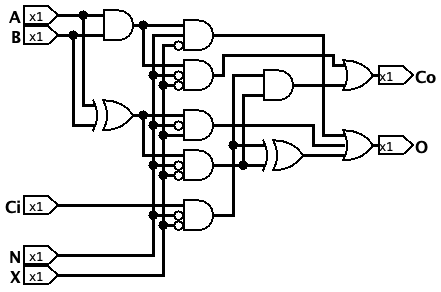
\includegraphics[scale=0.5]{ArithmeticLogicBit} \\
    \caption{ArithmeticLogicBit의 회로도}
    \label{fig:alb}
\end{figure}

\subsection{ArithmeticLogic}

ArithmeticLogic은 8비트 정수의 산술 연산과 논리 연산을 수행하는 부품이다.

ArithmeticLogic은 $A$, $B$, $I_A$, $I_B$, $I_O$, $B_e$, $N$, $X$, $C_i$의 입력 핀과
$O$, $C_o$의 출력 핀을 가지고 있다.
이중에서 $A$, $B$, $O$는 8비트 핀이다.
각각은 다음을 의미한다.

\begin{itemize}
    \item $A$ -- A. 연산의 첫 번째 인자가 될 수
    \item $B$ -- B. 연산의 두 번째 인자가 될 수
    \item $I_A$ -- Invert A. $A$의 결과를 반전하여 연산을 진행한다.
    \item $I_B$ -- Invert B. $\neg B$를 내부 두 번째 인자 입력에 논리합한다.
    \item $I_O$ -- Invert O. $O$의 결과를 반전하여 출력한다.
    \item $B_e$ -- B Enable. $B$를 내부 두 번째 인자 입력에 논리합한다.
    \item $N$ -- aNd enable. 두 수의 논리곱을 $O$에 출력한다.
    \item $X$ -- Xor enable. 두 수의 배타적 논리합을 $O$에 출력한다.
    \item $C_i$ -- Carry In. 가산 연산에 반영할 올림 비트
    \item $O$ -- Output. 연산의 결과
    \item $C_o$ -- Carry Out. 가산 연산에서 발생한 올림 비트
\end{itemize}

ArithmeticLogic은 입력되는 옵션에 따라 두 인자 $A$, $B$에 대한
$A$, $\neg A$, $A+1$, $A-1$, $A+B$, $A-B$, $-A$, $B-A$,
$A \veebar B$, $\neg(A \veebar B)$, $A\wedge B$, $\neg (A \wedge B)$, $A \vee B$, $\neg(A \vee B)$ 등을
계산할 수 있다.

ArithmeticLogic은 \tablename{} \ref{tab:al}와 같은 진리표를 가진다.
논리합($\vee$)과 산술합($+$) 연산에 주의해야 한다.

\begin{table}[p]
    \centering
    \begin{tabular}{cc|ccccccc|ll}
        $A$ & $B$ & $I_A$ & $I_B$ & $I_O$ & $B_e$ & $N$ & $X$ & $C_i$ & $O$ & $C_i$ \\
        \hline
        $A$ & $B$ & 0 & 0 & 0 & 0 & - & - & 0 & $A$ & 0 \\
        $A$ & $B$ & 0 & 0 & 0 & 0 & - & - & 1 & $A + 1$ & $\forall A$ \\
        $A$ & $B$ & 0 & 0 & 0 & 1 & 0 & 0 & 0 & $A + B$ & - \\
        $A$ & $B$ & 0 & 0 & 0 & 1 & 0 & 0 & 1 & $A + B + 1$ & - \\
        $A$ & $B$ & 0 & 0 & 0 & 1 & 0 & 1 & 0 & $A \veebar B$ & 0 \\
        $A$ & $B$ & 0 & 0 & 0 & 1 & 1 & 0 & 0 & $A \wedge B$ & 0 \\
        $A$ & $B$ & 0 & 0 & 1 & 0 & - & - & 0 & $\neg A$ & 0 \\
        $A$ & $B$ & 0 & 0 & 1 & 1 & 0 & 1 & 0 & $\neg(A \veebar B)$ & 0 \\
        $A$ & $B$ & 0 & 0 & 1 & 1 & 1 & 0 & 0 & $\neg(A \wedge B)$ & 0 \\
        $A$ & $B$ & 0 & 1 & 0 & 0 & 0 & 0 & 0 & $A - B - 1$ & $A > B$\\
        $A$ & $B$ & 0 & 1 & 0 & 0 & 0 & 0 & 1 & $A - B$ & $A \geq B$\\
        $A$ & $B$ & 0 & 1 & 0 & 1 & 0 & 0 & 0 & $A - 1$ & $\exists A$\\
        $A$ & $B$ & 0 & 1 & 1 & 0 & 0 & 0 & 0 & $B - A$ & $A > B$\\
        $A$ & $B$ & 0 & 1 & 1 & 0 & 0 & 0 & 1 & $B - A - 1$ & $A \geq B$\\
        $A$ & $B$ & 1 & 0 & 0 & 0 & 0 & 0 & 0 & $\neg A$ & 0 \\
        $A$ & $B$ & 1 & 0 & 0 & 0 & 0 & 0 & 1 & $-A$ & $\forall A$ \\
        $A$ & $B$ & 1 & 0 & 0 & 1 & 0 & 0 & 0 & $B - A - 1$ & - \\
        $A$ & $B$ & 1 & 0 & 0 & 1 & 0 & 0 & 1 & $B - A$ & - \\
        $A$ & $B$ & 1 & 1 & 0 & 0 & 0 & 0 & 0 & $-A-B-2$ & - \\
        $A$ & $B$ & 1 & 1 & 0 & 0 & 0 & 0 & 1 & $-A-B-1$ & - \\
        $A$ & $B$ & 1 & 1 & 0 & 0 & 1 & 0 & 0 & $\neg(A \vee B)$ & - \\
        $A$ & $B$ & 1 & 1 & 0 & 1 & 0 & 0 & 0 & $-A-2$ & $\neg \forall A$ \\
        $A$ & $B$ & 1 & 1 & 0 & 1 & 0 & 0 & 1 & $-A-1$ & 1 \\
        $A$ & $B$ & 1 & 1 & 1 & 0 & 1 & 0 & 0 & $A \vee B$ & 0 \\
    \end{tabular}
    \caption{ArithmeticLogic}
    \label{tab:al}
\end{table}

\figurename{} \ref{fig:al}은 ArithmeticLogic의 회로도이다.

\begin{figure}[p]
    \centering
    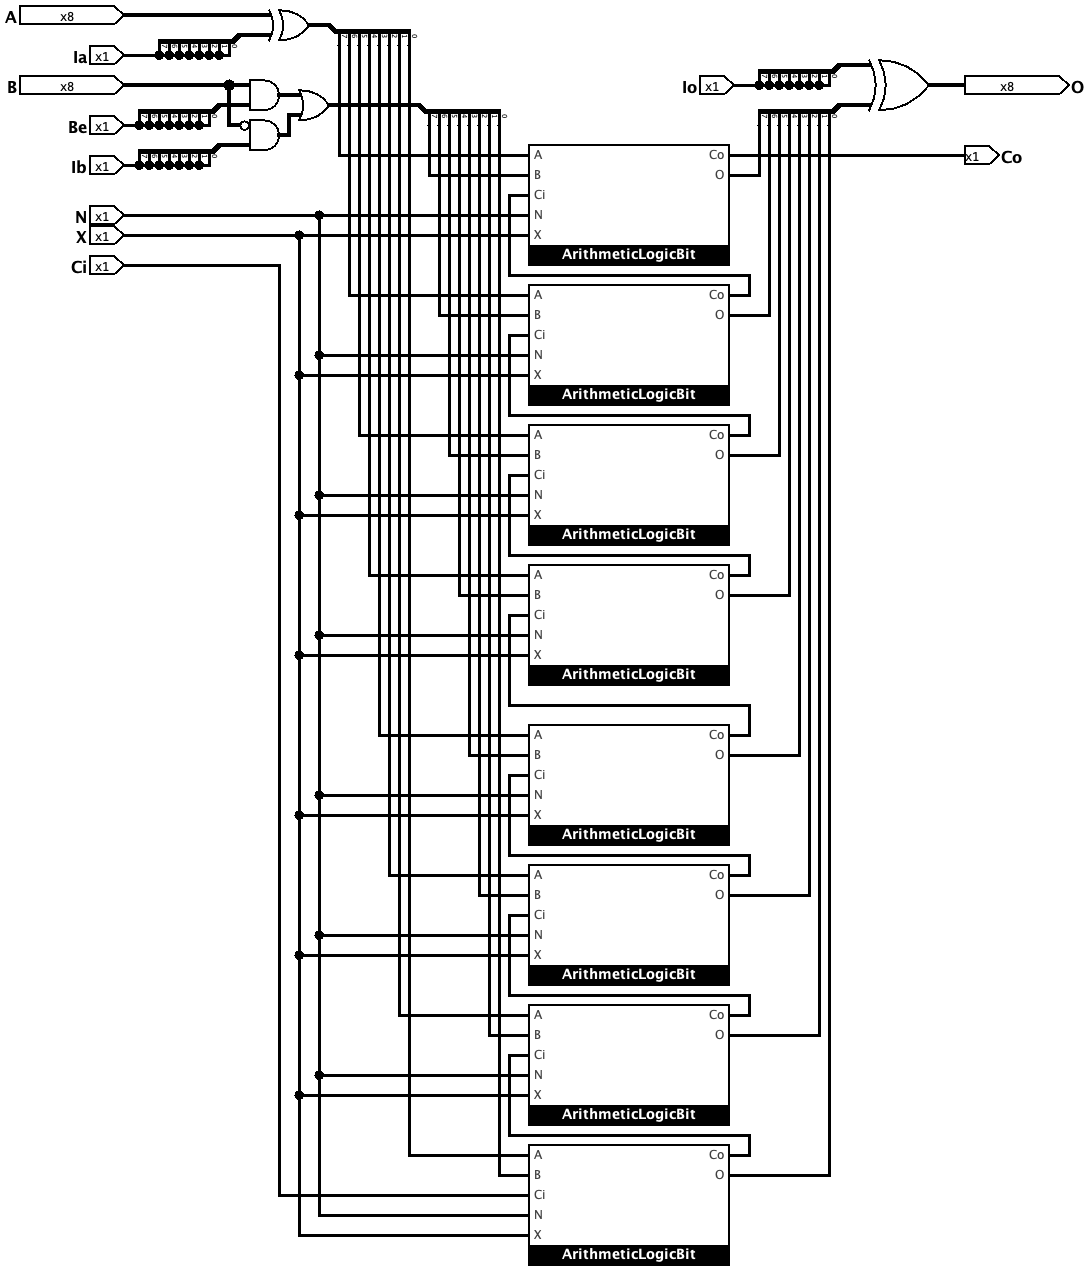
\includegraphics[scale=0.35]{ArithmeticLogic} \\
    \caption{ArithmeticLogic의 회로도}
    \label{fig:al}
\end{figure}

\pagebreak

\subsection{Shiftre}

Shiftre는 입력된 값에 대한 1회 좌측·우측 시프트 연산 결과를 출력하는
부품이다.

Shiftre는 $I$, $S$, $R$, $L$의 입력 핀과
$O$, $O_l$, $O_r$의 출력 핀을 가지고 있다.
이중에서 $I$, $O$는 8비트 핀이다.
각각은 다음을 의미한다.

\begin{itemize}
    \item $I$ -- Input. 시프트 연산을 수행할 정수
    \item $E$ -- Enable. 시프트 연산 수행의 여부.
        0으로 설정된 경우에는 연산을 수행하지 않고,
        1로 설정된 경우에는 연산을 수행한다.
    \item $R$ -- Right. 시프트 방향을 오른쪽으로 설정한다.
        0으로 설정된 경우에는 왼쪽 시프트를 수행한다.
    \item $L$ -- Logical. 오른쪽 시프트를 수행하는 경우에,
        논리적 시프트와 산술적 시프트 중에서 선택한다.
        0으로 설정된 경우에는 산술적 시프트를 수행하고,
        1로 설정된 경우에는 논리적 시프트를 수행한다.
    \item $O$ -- Output. 시프트 결과
    \item $O_l$ -- Overflow Left. 왼쪽 시프트 수행 중에 오버플로우가 발생함
    \item $O_r$ -- Overflow Right. 오른쪽 시프트 수행 중에 오버플로우가 발생함
\end{itemize}

\tablename{} \ref{tab:shr}은 Shiftre의 표이다.

\begin{table}[h]
    \centering
    \begin{tabular}{c|ccc|ccc}
        $I$ & $E$ & $R$ & $L$ & $O$ & $O_l$ & $O_r$ \\
        \hline
        \texttt{abcd efgh} & 0 & - & - & \texttt{abcd efgh} & 0 & 0 \\
        \texttt{abcd efgh} & 1 & 0 & - & \texttt{bcde fgh0} & \texttt a & 0 \\
        \texttt{abcd efgh} & 1 & 1 & 0 & \texttt{aabc defg} & 0 & \texttt h \\
        \texttt{abcd efgh} & 1 & 1 & 1 & \texttt{0abc defg} & 0 & \texttt h \\
    \end{tabular}
    \caption{Shiftre의 진리표}
    \label{tab:shr}
\end{table}

\figurename{} \ref{fig:shr}은 Shiftre의 회로도이다.

\begin{figure}[p]
    \centering
    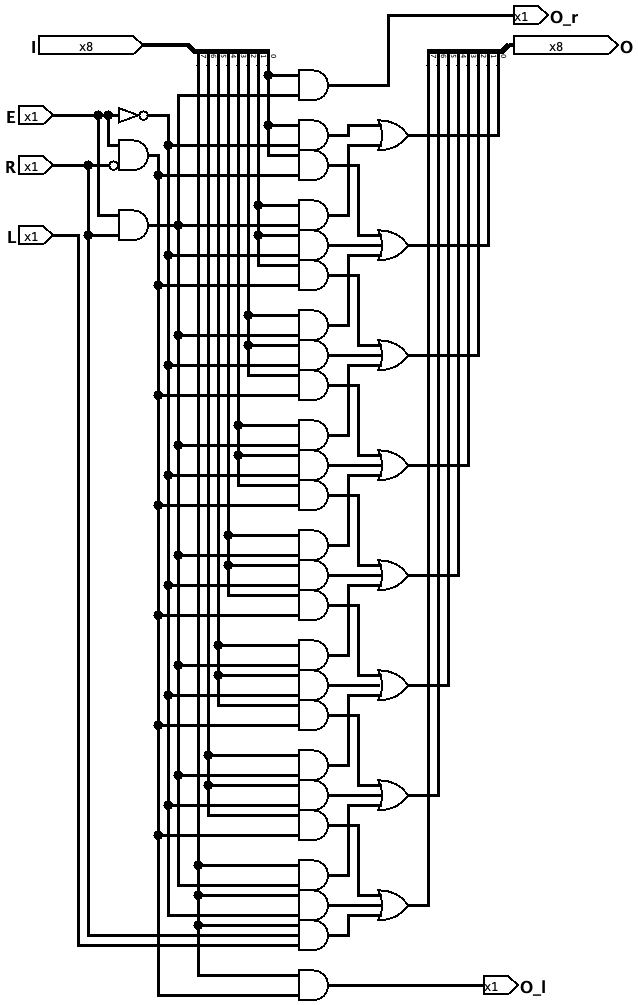
\includegraphics[scale=0.5]{Shiftre} \\
    \caption{Shiftre의 회로도}
    \label{fig:shr}
\end{figure}

\pagebreak

\subsection{OpCodeToFlags}

OpCodeToFlags는 4비트 연산자 코드를 ArithmeticLogic 플래그로 변환해주는
부품이다.

OpCodeToFlags는 $O_c$의 입력 핀과
$I_A$, $I_B$, $I_O$, $B_e$, $N$, $X$, $C_i$, $E$, $R$, $L$ 출력 핀을 가지고 있다.
이중에서 $O_c$는 4비트 입력 핀이다.
$I_A$, $I_B$, $I_O$, $B_e$, $N$, $X$, $C_i$는 ArithmeticLogic에 입력되는 핀이고
$E$, $R$, $L$는 Shiftre에 입력되는 핀이다.

OpCodeToFlags의 진리표는 \tablename{} \ref{tab:octf}과 같다.
기울인꼴로 표현된 것은 무관조건이다.

\begin{table}[h]
    \centering
    \begin{tabular}{cl||ccccccc|ccc}
        $O_c$ & 연산자 & $I_A$ & $I_B$ & $I_O$ & $B_e$ & $N$ & $X$ & $C_i$ & $E$ & $R$ & $L$ \\
        \hline
        \texttt{0} & A    & 0 & 0 & 0 & 0 & \textit 0 & \textit 1 & 0 & 0 & \textit 0 & \textit 0 \\
        \texttt{1} & NOT  & 1 & 0 & 0 & 0 & \textit 0 & \textit 1 & 0 & 0 & \textit 0 & \textit 1 \\
        \texttt{2} & NEG  & 1 & 0 & 0 & 0 & \textit 1 & \textit 0 & 1 & 0 & \textit 0 & \textit 0 \\
        \texttt{3} & SHL  & 0 & 0 & 0 & 0 & \textit 1 & \textit 0 & 0 & 1 & 0 & \textit 1\\
        \texttt{4} & INC  & 0 & 0 & 0 & 0 & \textit 0 & \textit 0 & 1 & 0 & \textit 1& \textit 0 \\
        \texttt{5} & DEC  & 0 & 1 & 0 & 1 & 0 & 0 & 0 & 0 & \textit 1& \textit 1\\
        \texttt{6} & ADD  & 0 & 0 & 0 & 1 & 0 & 0 & 0 & 0 & \textit 1& \textit 0 \\
        \texttt{7} & SUB  & 0 & 1 & 0 & 0 & 0 & 0 & 1 & 0 & \textit 1& \textit 1\\
        \texttt{8} & XOR  & 0 & 0 & 0 & 1 & 0 & 1 & 0 & 0 & \textit 0 & \textit 0 \\
        \texttt{9} & XNOR & 0 & 0 & 1 & 1 & 0 & 1 & 0 & 0 & \textit 0 & \textit 1\\
        \texttt{A} & AND  & 0 & 0 & 0 & 1 & 1 & 0 & 0 & 0 & \textit 0 & \textit 0 \\
        \texttt{B} & NAND & 0 & 0 & 1 & 1 & 1 & 0 & 0 & 0 & \textit 0 & \textit 1\\
        \texttt{C} & OR   & 1 & 1 & 1 & 0 & 1 & 0 & 0 & 0 & \textit 1& \textit 0 \\
        \texttt{D} & NOR  & 1 & 1 & 0 & 0 & 1 & 0 & 0 & 0 & \textit 1& \textit 1\\
        \texttt{E} & ASR  & 0 & 0 & 0 & 0 & \textit 1& \textit 0 & 0 & 1 & 1 & 0 \\
        \texttt{F} & LSR  & 0 & 0 & 0 & 0 & \textit 1& \textit 0 & 0 & 1 & 1 & 1 \\
    \end{tabular}
    \caption{OpCodeToFlags의 진리표}
    \label{tab:octf}
\end{table}

OpCodeToFlags의 회로도는 \figurename{} \ref{fig:octf}과 같다.

\begin{figure}[p]
    \centering
    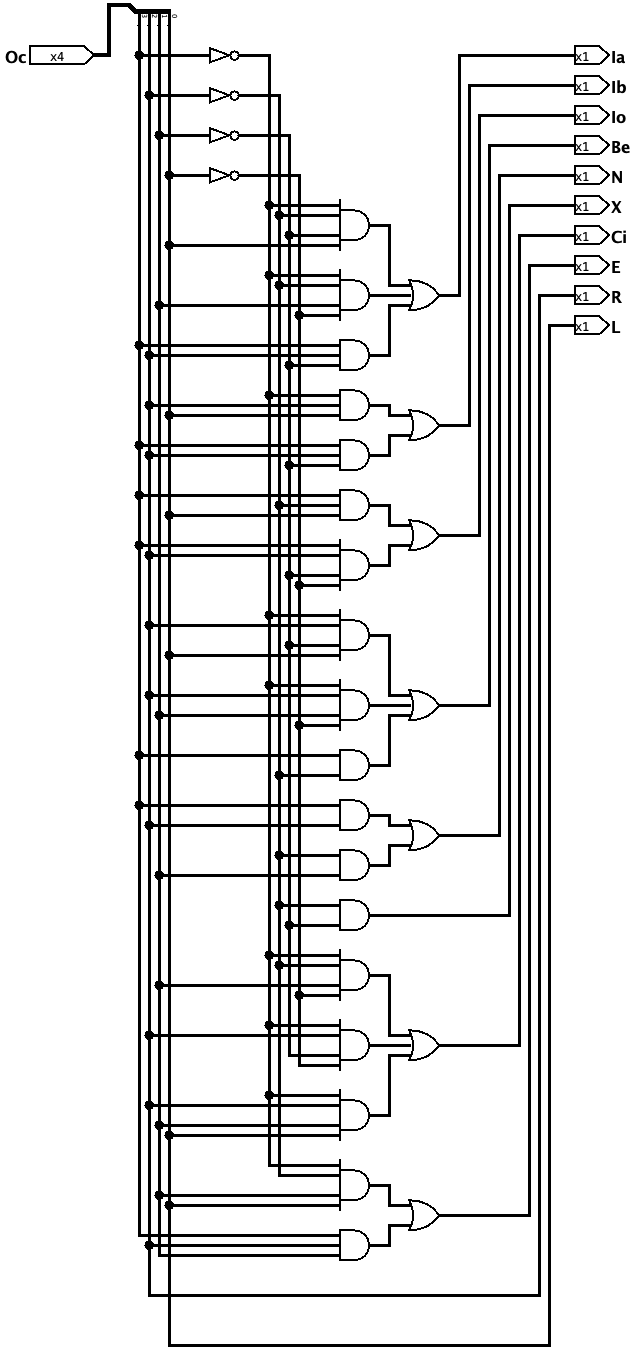
\includegraphics[scale=0.35]{OpCodeToFlags} \\
    \caption{OpCodeToFlags의 회로도}
    \label{fig:octf}
\end{figure}

\pagebreak

\subsection{ALU}

ALU는 Arithmetic Logical Unit의 약자로,
산술 연산과 논리 연산을 수행하고 그 결과를 출력하는 부품이다.

ALU는 $A$, $B$, $O_c$의 입력 핀과
$O$, $F_v$, $F_c$, $F_s$, $F_z$의 출력 핀으로 이루어져 있다.
이중 $A$, $B$, $O$는 8비트 핀이고, $O_c$는 4비트 핀이다.
각각이 의미하는 바는 다음과 같다.

\begin{itemize}
    \item $A$ -- A. 연산의 첫 번째 인자
    \item $B$ -- B. 연산의 두 번째 인자
    \item $O_c$ -- Operation Code. 연산의 종류.
        $O_c$ 값에 따른 연산의 종류는 \tablename{} \ref{tab:aluopc}에서 설명되어있다.
    \item $O$ -- Output. 연산의 결과.
    \item $F_v$ -- Flag of oVerflow. 시프트 연산 중에 오버플로우가 발생하면
        활성화되는 플래그
    \item $F_c$ -- Flag of Carry. 가감산 연산 중에 올림수가 발생하면
        활성화되는 플래그
    \item $F_s$ -- Flag of Sign. 연산 결과의 부호를 나타내는 플래그.
        $O < 0$이면 활성화된다.
    \item $F_z$ -- Flag of Zero. 연산 결과가 $0$이면 활성화되는 플래그
\end{itemize}

\figurename{} \ref{fig:alu}는 ALU의 회로도이다.

\begin{figure}[h]
    \centering
    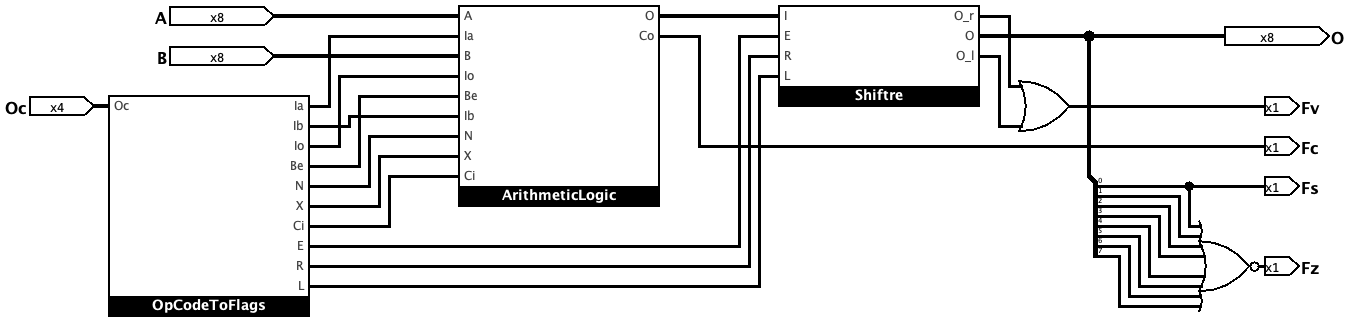
\includegraphics[scale=0.25]{ALU}
    \caption{ALU 회로도}
    \label{fig:alu}
\end{figure}

$O_c$ 값에 따라 수행되는 연산은 다음 \tablename{} \ref{tab:aluopc}과 같다.

\begin{table}
    \centering
    \begin{tabular}{rl|ll}
        $O_c$ & 연산 이름 & 연산 & 설명\\
        \hline
        \texttt 0 & A    & $A$ & A \\
        \texttt 1 & NOT  & $\neg A$ & NOT \\
        \texttt 2 & NEG  & $- A$ & NEGative \\
        \texttt 3 & SHL  & $A \ll 1$ & SHift Left \\
        \texttt 4 & INC  & $A + 1$ & INCrease \\
        \texttt 5 & DEC  & $A - 1$ & DECrease \\
        \texttt 6 & ADD  & $A + B$ & ADD \\
        \texttt 7 & SUB  & $A - B$ & SUBtract \\
        \texttt 8 & XOR  & $A \veebar B$ & eXclusive OR \\
        \texttt 9 & XNOR & $\neg (A \veebar B)$ & eXclusive Not OR \\
        \texttt A & AND  & $A \wedge B$ & AND \\
        \texttt B & NAND & $\neg (A \wedge B)$ & Not AND \\
        \texttt C & OR   & $A \vee B$ & OR \\
        \texttt D & NOR  & $\neg (A \vee B)$ & Not OR \\
        \texttt E & ASR  & $A \sim\gg 1$ & Arithmetic Shift Right \\
        \texttt F & LSR  & $A \gg 1$ & Logical Shift Right \\
    \end{tabular}
    \caption{ALU의 $O_c$ 값에 따라 계산되는 연산}
    \label{tab:aluopc}
\end{table}

\pagebreak

\subsection{Countre}

Countre는 매 클락마다 현재 수의 다음 수를 계산하는 부품이다.
Countre는 현재 실행하고 있는 명령어의 주소를 계산하는 데에 사용된다.

Countre는 $I$, $E_w$, $\textit{c}$의 입력 핀과
$O$, $c_o$의 출력 핀을 가지고 있다.
이중에서 $I$, $O$는 8비트 핀이다.
각각은 다음을 의미한다.

\begin{itemize}
    \item $I$ -- Input. $\overline{E_w}$일 때에 카운터에 적재할 값
    \item $E_w$ -- Enable $\overline{\textrm{Write}}$. 카운터를 실행한다.
        0으로 설정된 경우에는 $I$의 값을 카운터에 적재한다.
    \item $c$ -- Clock. 시스템 클락
    \item $O$ -- Output. 카운터에 적재되어있는 값
    \item $c_o$ -- Clock Overflowed. 카운터 확장을 위해 사용되는 클락.
        $\overline{O_7}$의 값과 같다.
\end{itemize}

\figurename{} \ref{fig:ctr}은 Countre의 회로도이고,
\tablename{} \ref{tab:ctr}은 Countre의 표이다.

\begin{figure}[h]
    \centering
    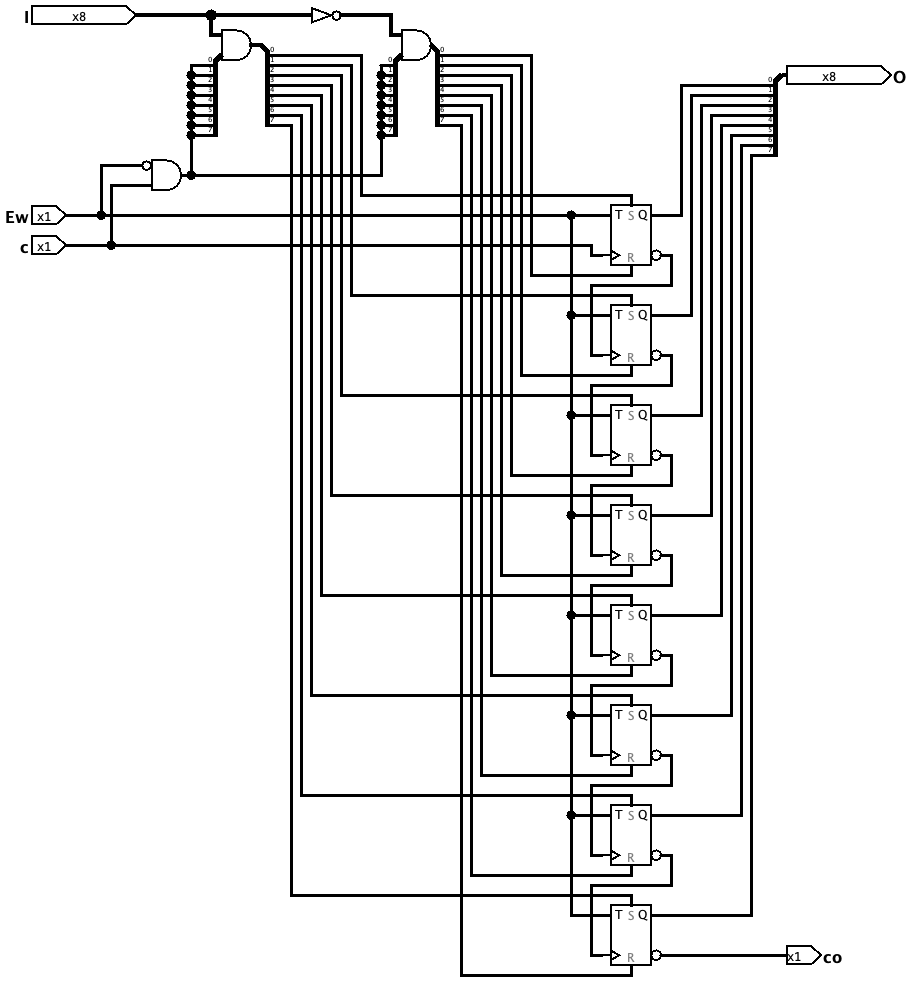
\includegraphics[scale=0.35]{Countre}
    \caption{Countre의 회로도}
    \label{fig:ctr}
\end{figure}

\begin{table}[h]
    \centering
    \begin{tabular}{cc|c}
        $I$ & $E_w$ & $O$ \\
        \hline
        $I$ & 0 & $O+1$ \\
        $I$ & 1 & $I$ \\
    \end{tabular}
    \caption{Countre의 표}
    \label{tab:ctr}
\end{table}

\section{CPU}

CPU는 Central Processing Unit의 약자로,
메모리에서 명령어를 읽어 해석하여 실행하는 부품이다.

CPU에는 메모리를 연결하여 프로그래밍할 수 있으며,
프로그래밍 방법에 대해서는 \ref{sec:machlang}장을 참고한다.

\subsection{제어 신호}

\begin{enumerate}
    \setcounter{enumi}{-1}
    \item \texttt{LO} -- aLu Out. ALU의 출력을 버스에 적재한다.
    \item \texttt{AI} -- A register In. 버스의 내용을 A 레지스터에 적재한다.
    \item \texttt{CI} -- aCcumulator In. 버스의 내용을 누산기에 적재한다.
    \item \texttt{OI} -- Opcode register In. 버스의 내용 중 하위 4bit를 OR에 적재한다.
    \item \texttt{PW} -- Program counter Write. 버스의 내용을 PC에 적재한다.
    \item \texttt{PO} -- Program counter Out. PC의 내용을 버스에 적재한다.
    \item \texttt{DI} -- aDdress register In. 버스의 내용을 MAR에 적재한다.
    \item \texttt{MO} -- Memory Out. 메모리의 내용을 버스에 적재한다.
    \item \texttt{MI} -- Memory In. 버스의 내용을 메모리에 적재한다.
    \item \texttt{PE} -- Program counter Enable. PC의 내용을 1 증가시킨다.
    \item \texttt{II} -- Instruction register In. 메모리의 내용을 IR에 적재한다.
    \item \texttt{HLT} -- HaLT. 클락을 비활성화한다.
    \item \texttt{AO} -- A register Out. A 레지스터의 내용을 버스에 적재한다.
    \item \texttt{CO} -- aCcumulator Out. 누산기의 내용을 버스에 적재한다.
\end{enumerate}

\subsection{명령어 해독기}

명령어 해독기는 인스트럭션, 플래그, 인스트럭션 카운터의 출력을 받아
그에 맞는 마이크로인스트럭션을 출력하는 부품이다.

CPU에서는 8b의 인스트럭션, 4b의 플래그, 3b의 인스트럭션 카운터 출력을 주소로 받아
8bit 출력을 내보내는 ROM 2개가 사용되었다.

\section{기계어}
\label{sec:machlang}

기계어는 CPU를 프로그래밍하기 위한 언어이다.
CPU는 메모리에서 기계어를 읽어 기계어에 해당하는
제어 신호를 순차적으로 설정한다.
설정된 제어 신호에 따라 클락마다 하나의 동작씩 수행되는 것이다.
CPU는 한 명령어당 최대 8개의 제어 신호 동작을 수행할 수 있게
설계되었다.

\subsection{명령어}

명령어(command)는 인스트럭션(instruction)과
인자(argument)로 나누어지는 추상화된 동작에 대한 명세이다.
인스트럭션은 8비트로 구성되며, 인자는 명령어의 종류에 따라
가변적으로 길이가 변한다.

마이크로인스트럭션(microinstruction, \textmu i)이란
하나의 인스트럭션을 이루는 8가지의 작은 동작들을 의미한다.
하나의 마이크로인스트럭션은 제어 신호에 대한 활성화 유무로 이루어져 있다.

하나의 인스트럭션은 적재, 증가, 실행으로 나누어져 있다.
적재와 증가부분은 함께 2\textmu i으로 이루어져 있으므로
실행 부분은 최대 6개의 \textmu i으로 이루어진다.

적재는 PC의 값을 메모리 주소 레지스터(Memory Addrees Register, MAR)에
적재하고 메모리 상의 인스트럭션을 인스트럭션 레지스터(Instruction Register, IR)에
적재하는 동작이다. 이는 \texttt{PO DI}, \texttt{MO II}를 각각 실행하는 것으로 수행된다.
증가는 다음 명령어 실행을 위해 프로그램 카운터(PC)를 증가하는 동작이다.
이는 \texttt{PE} 신호를 활성화하는 것으로 수행된다.
이때, \texttt{MO II}와 \texttt{PE}는 함께 실행할 수 있으므로
적재와 증가를 2\textmu i만에 수행할 수 있게 된다.

\subsubsection{\texttt{00} -- NOP}

NOP는 No OPeration의 약자로, 아무런 동작을 수행하지 않고
다음 명령어를 실행하게 하는 명령어이다.
명령어의 인스트럭션은 \texttt{00}이고 명령어의 길이는 1B이다.

NOP 명령어는 다음 마이크로인스트럭션들로 이루어진다.

\begin{enumerate}
    \item \texttt{PO DI(0060), MO II PE(0680)} -- 다음 명령어 실행을 준비한다.
    \setcounter{enumi}{2}
\end{enumerate}

\subsubsection{\texttt{01} -- LDI}

LDI는 LoaD Immediate의 약자로, 뒤에 따라오는 1B의 자료를
A 레지스터에 저장하는 명령어이다.
명령어의 인스트럭션은 \texttt{01}이고 명령어의 길이는 2B이다.

LDI 명령어는 다음 마이크로인스트럭션들로 이루어진다.

\begin{enumerate}
    \item \texttt{PO DI(0060), MO II PE(0680)} -- 다음 명령어 실행을 준비한다.
    \setcounter{enumi}{2}
    \item \texttt{PO DI(0060)} -- 1 올린 PC의 내용을 MAR에 저장한다.
    \item \texttt{AI MO PE(0282)} -- 메모리에 써있는 내용을 A 레지스터에 옮기고
        PC의 내용을 1 더 올린다.
\end{enumerate}

\subsubsection{\texttt{02} -- STA}

STA는 STore A register의 약자로, A 레지스터에 있는 값을
뒤에 따라오는 1B의 주소에 해당하는 메모리에 저장하는 명령어이다.
명령어의 인스트럭션은 \texttt{02}이고 명령어의 길이는 2B이다.

STA 명령어는 다음 마이크로인스트럭션들로 이루어진다.

\begin{enumerate}
    \item \texttt{PO DI(0060), MO II PE(0680)} -- 다음 명령어 실행을 준비한다.
    \setcounter{enumi}{2}
    \item \texttt{PO DI(0060)} -- 1 올린 PC의 내용을 MAR에 저장한다.
    \item \texttt{MO DI(00C0)} -- 메모리에 써있는 주소를 MAR에 저장한다.
    \item \texttt{AO MI PE(1300)} -- A 레지스터의 값을 메모리에 저장하고
        PC의 내용을 1 더 올린다.
\end{enumerate}

\subsubsection{\texttt{03} -- LDA}

LDA는 LoaD A register from memory의 약자로, 뒤에 따라오는 1B의 주소에 해당하는
메모리의 값을 A 레지스터에 불러오는 명령어이다.
명령어의 인스트럭션은 \texttt{03}이고 명령어의 길이는 2B이다.

LDA 명령어는 다음 마이크로인스트럭션들로 이루어진다.

\begin{enumerate}
    \item \texttt{PO DI(0060), MO II PE(0680)} -- 다음 명령어 실행을 준비한다.
    \setcounter{enumi}{2}
    \item \texttt{PO DI(0060)} -- 1 올린 PC의 내용을 MAR에 저장한다.
    \item \texttt{MO DI(00C0)} -- 메모리의 내용을 MAR에 저장한다.
    \item \texttt{MO AI PE(0282)} -- 메모리의 내용을 A 레지스터에 저장하고,
        PC의 내용을 1 더 올린다.
\end{enumerate}

\subsubsection{\texttt{04} -- STC}

STC는 STore aCcumulator의 약자로, 누산기에 있는 값을
뒤에 따라오는 1B의 주소에 해당하는 메모리에 저장하는 명령어이다.
명령어의 인스트럭션은 \texttt{04}이고 명령어의 길이는 2B이다.

STC 명령어는 다음 마이크로인스트럭션들로 이루어진다.

\begin{enumerate}
    \item \texttt{PO DI(0060), MO II PE(0680)} -- 다음 명령어 실행을 준비한다.
    \setcounter{enumi}{2}
    \item \texttt{PO DI(0060)} -- 1 올린 PC의 내용을 MAR에 저장한다.
    \item \texttt{MO DI(00C0)} -- 메모리에 써있는 주소를 MAR에 저장한다.
    \item \texttt{CO MI PE(2300)} -- 누산기의 값을 메모리에 저장하고
        PC의 내용을 1 더 올린다.
\end{enumerate}

\subsubsection{\texttt{05} -- LIC}

LIC는 Load Immediate aCcumulator의 약자로,
뒤에 따라오는 1B의 값을 누산기에 저장한다.
명령어의 인스트럭션은 \texttt{05}이고 명령어의 길이는 2B이다.

LIC 명령어는 다음 마이크로인스트럭션들로 이루어진다.

\begin{enumerate}
    \item \texttt{PO DI(0060), MO II PE(0680)} -- 다음 명령어 실행을 준비한다.
    \setcounter{enumi}{2}
    \item \texttt{PO DI(0060)} -- 1 올린 PC의 내용을 MAR에 저장한다.
    \item \texttt{CI MO PE(0284)} -- 메모리에 써있는 내용을 누산기에 옮긴다.
\end{enumerate}

\subsubsection{\texttt{06} -- SOC}

SOC는 Select OpCode의 약자로, OR의 값을 뒤에 따라오는 1B 값으로 바꾼다.
단, OR이 한번에 4bit의 값만 적재하므로 1B의 아래 4bit만 적재한다.
명령어의 인스트럭션은 \texttt{06}이고 명령어의 길이는 2B이다.

SOC 명령어는 다음 마이크로인스트럭션들로 이루어진다.

\begin{enumerate}
    \item \texttt{PO DI(0060), MO II PE(0680)} -- 다음 명령어 실행을 준비한다.
    \setcounter{enumi}{2}
    \item \texttt{PO DI(0060)} -- 1 올린 PC의 내용을 MAR에 저장한다.
    \item \texttt{MO OI PE(0288)} -- 메모리의 내용을 OR에 저장하고,
        PC의 내용을 1 더 올린다.
\end{enumerate}

\subsubsection{\texttt{07} -- CMP}

ADD는 A 레지스터의 값과 뒤에 따라오는 1B의 주소에 해당하는 메모리의 값을
OR에 저장된 연산에 따라 계산하고 누산기에 적재하는 명령어이다.
명령어의 인스트럭션은 \texttt{06}이고 명령어의 길이는 2B이다.

CMP 명령어는 다음 마이크로인스트럭션들로 이루어진다.

\begin{enumerate}
    \item \texttt{PO DI(0060), MO II PE(0680)} -- 다음 명령어 실행을 준비한다.
    \setcounter{enumi}{2}
    \item \texttt{PO DI(0060)} -- 1 올린 PC의 내용을 MAR에 저장한다.
    \item \texttt{MO DI(00C0)} -- 메모리의 내용을 MAR에 저장한다.
    \item \texttt{MO CI (0084)} -- 메모리의 내용을 누산기에 저장한다.
    \item \texttt{LO CI PE (0205)} -- ALU의 내용을 누산기에 저장하고,
        PC의 내용을 1 더 올린다.
\end{enumerate}

\subsubsection{\texttt{08} -- JMP}

JMP는 JuMP의 약자로, 뒤에 따라오는 주소에 있는 명령어를 실행한다.
명령어의 인스트럭션은 \texttt{08}이고 명령어의 길이는 2B이다.

JMP 명령어는 다음 마이크로인스트럭션들로 이루어진다.

\begin{enumerate}
    \item \texttt{PO DI(0060), MO II PE(0680)} -- 다음 명령어 실행을 준비한다.
    \setcounter{enumi}{2}
    \item \texttt{PO DI(0060)} -- 1 올린 PC의 내용을 MAR에 저장한다.
    \item \texttt{MO PW(0090)} -- 메모리의 내용을 PC에 저장한다.
\end{enumerate}

\subsubsection{\texttt{FF} -- HLT}

HLT는 HaLT의 약자로, 컴퓨터의 동작을 종료하는 명령어이다.
명령어의 인스트럭션은 \texttt{FF}이고 명령어의 길이는 1B이다.

HLT 명령어는 다음 마이크로인스트럭션들로 이루어진다.

\begin{enumerate}
    \item \texttt{PO DI(0060), MO II PE(0680)} -- 다음 명령어 실행을 준비한다.
    \setcounter{enumi}{2}
    \item \texttt{HLT(0800)} -- 컴퓨터를 정지한다.
\end{enumerate}

\end{document}
